\documentclass[12pt,tikz]{standalone}

\usepackage{graphicx}
\usetikzlibrary{positioning}
\usetikzlibrary{automata}
\begin{document}

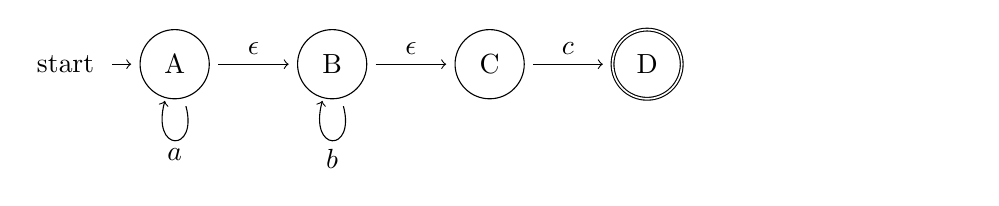
\begin{tikzpicture}[->, draw, black, auto, shorten >=3pt, shorten <=3pt, node distance = 2cm]
  \node at (10, 0) (dummy) {};

  \node[initial,state] (A) {A};
  \node[state] (B) [right of = A] {B};
  \node[state] (C) [right of = B] {C};
  \node[state,accepting] (D) [right of = C] {D};

  \path
  (A) edge [loop below] node {$a$} (A)
  (A) edge node {$\epsilon$} (B)
  (B) edge [loop below] node {$b$} (B)
  (B) edge node {$\epsilon$} (C)
  (C) edge node {$c$} (D);
\end{tikzpicture}

\end{document}
